\subsection*{Seguretat de dades}
\addcontentsline{toc}{subsection}{Seguretat de dades}


En general, els serveis financers solen implementar mesures de seguretat estàndard per protegir la informació financera i les transaccions. Aquestes mesures poden incloure:

\begin{itemize}
    \item Xifratge de dades en trànsit: S'utilitza xifratge de capa de transport (TLS o SSL) per protegir la informació mentre es transmet entre el dispositiu de l'usuari i els servidors del servei.
    \item Xifratge de Dades en Repòs: La informació emmagatzemada als servidors es xifra per protegir-la contra l'accés no autoritzat.
    \item Autenticació de Dos Factors: Per accedir al compte o fer transaccions, es pot requerir l'autenticació de dos factors, com ara la combinació d'una contrasenya amb un codi enviat al telèfon mòbil de l'usuari.
\end{itemize}



\subsection*{Diferents maneres de afectuar el pagament via digital}
\addcontentsline{toc}{subsection}{Diferents maneres de afectuar el pagament via digital}



\subsubsection*{Tarjeta Bancari}


La primera targeta bancària generalment s'atribueix a la targeta Diners Club, que va ser creada el 1950 per Frank McNamara, un empresari nord-americà, i Alfred Bloomingdale, un empresari. La idea darrere de la targeta Diners Club era proporcionar als clients una forma convenient de pagar a restaurants sense necessitat de portar efectiu.

La targeta Diners Club Va ser un precursor important de les targetes de crèdit modernes, i el seu èxit va inspirar la creació daltres targetes bancàries en els anys següents. Poc després, el 1958, es va llançar la targeta American Express, seguida per la introducció de targetes Visa i MasterCard als anys 1960.

\begin{figure}[h]
    \centering
    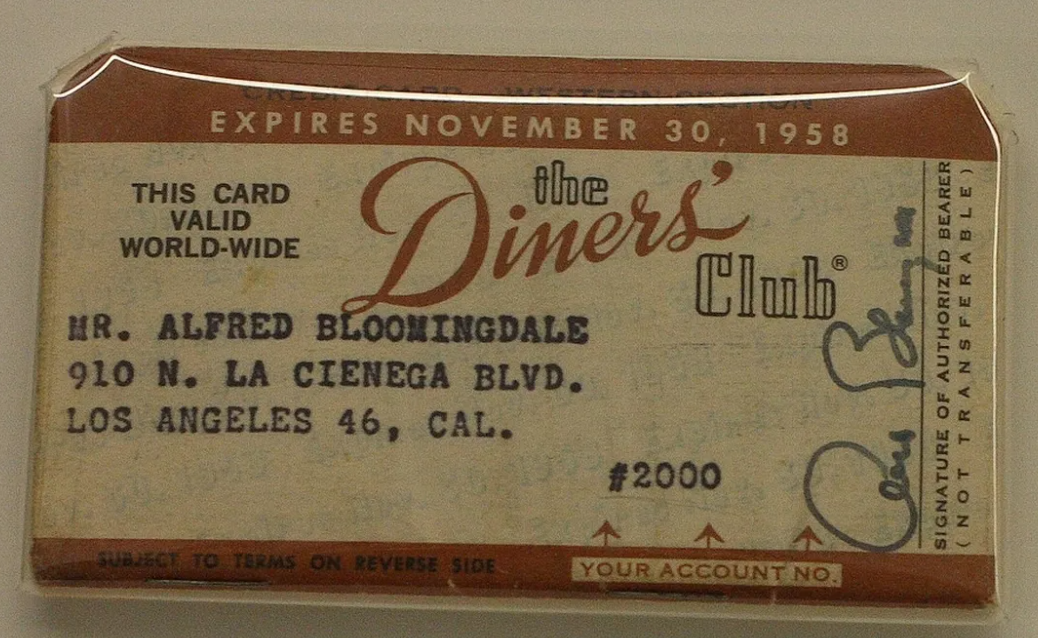
\includegraphics[width=5cm]{primeratarjeta.png}
    \caption{Primera tarjeta bancaria}
\end{figure}  


L'abril del 1971 es llança la primera targeta bancària a Espanya per part del Banc de Bilbao. En aliança amb BankAmericard, aquesta primera targeta de crèdit permetia el pagament total a final de mes o l'ajornament amb un percentatge del 10\% del saldo disposat, comptant amb un límit màxim de 25.000 pessetes.


La targeta Diners Club funcionava amb banda magnètica, que conté informació vital, com ara el número de compte i la informació del compte del titular. Quan la targeta llisca o s'insereix en un terminal de pagament, la banda magnètica transfereix aquesta informació al sistema de processament de pagaments, les quals poden ser fàcilment robats i clonats. 

Actualment, moltes targetes incorporen tecnologies més avançades com els xips EMV, que contenen un xip que crea un codi únic per a cada transacció, un que no pot ser clonat i que queda inutilitzat un cop completada la transacció.

És important destacar que encara que la banda magnètica ha estat una tecnologia comuna en targetes durant dècades, es considera menys segura en comparació amb altres tecnologies més recents. La transició cap a tecnologies més segures com EMV ha estat un esforç global per reduir el frau relacionat amb targetes. Tot i que la banda magnètica encara s'utilitza en moltes targetes, especialment en àrees on la infraestructura de pagaments pot ser més antiga. Ara, les targetes amb xip i PIN són més segures tant pels comerços com pels consumidors.
(Pagament sense contacte)
(fraudes de tarjeta banda magnetica)


\subsubsection*{Bizum}


Bizum és un proveïdor de serveis de pagament d'Espanya, fruit de la col·laboració de 34 entitats bancàries del país, per crear un sistema de pagaments instantanis entre particulars i de compres a comerços. El 2019 Bizum va superar els 6 milions d'usuaris. Ja l'agost del 2020 va arribar a 10 milions d'usuaris. El 2021 va arribar als 15 milions d'usuaris.

Bizum només està disponible a Espanya. Es pot fer Bizum a un altre país, però cal tenir un compte bancari en una entitat espanyola. Aquest és l'únic requisit per continuar fent servir Bizum fora d'Espanya. I de la mateixa manera només podràs fer pagaments amb Bizum a números vinculats a un compte d'un banc espanyol.

\subsubsection*{servei de pagament tercers}

Samsung Pay o Apple Pay Alipay









